\documentclass[conference,a4paper]{IEEEtran}

\usepackage{amsmath,amssymb,amsfonts}
\usepackage{graphicx}
\usepackage{textcomp}
\usepackage{xcolor}
\usepackage{booktabs}
\usepackage{array}
\usepackage{listings}
\usepackage{url}
\usepackage{hyperref}
\usepackage{cite}
\usepackage{tikz}
\usetikzlibrary{positioning,fit,arrows.meta}

\graphicspath{{figures/}{../results/figures/}}

\lstset{
	basicstyle=\ttfamily\footnotesize,
	keywordstyle=\color{blue}\bfseries,
	commentstyle=\color{gray}\itshape,
	stringstyle=\color{red},
	numbers=left,
	numberstyle=\tiny\color{gray},
	numbersep=5pt,
	frame=single,
	breaklines=true,
	captionpos=b,
	tabsize=4
}

\begin{document}

\title{How Much Downtime Do Replicas, Probes and Rolling Updates Remove? A Measurement Study on a Local Kubernetes Cluster\\[10pt]
	{\normalsize SEN421 --- Cloud Architecture and Services, Course Project, Fall 2026}
}

\author{\IEEEauthorblockN{Ahmet Seyid Bilal Demircan}
	\IEEEauthorblockA{\textit{Department of Computer Engineering}\\
		\textit{Istanbul Ayd\i n University}\\
		Istanbul, Turkey \\
		Student ID: B2305.010146 \\
		aseyiddemircan@stu.aydin.edu.tr}
}

\maketitle

\begin{abstract}
Kubernetes is often described as self-healing and able to update applications without downtime, but these properties depend on how a workload is configured. This Topic 8, Part A study measures how much user-visible downtime a pod failure and a version update cause on a small Kubernetes deployment, how much of it is removed by multiple replicas with readiness probes and by the RollingUpdate strategy, and how quickly the Horizontal Pod Autoscaler reacts at a 50 percent and an 80 percent CPU target. A Flask API with a Redis backend was deployed on a local three-node kind cluster, and each of three experiments compared two configurations over three repetitions, measured by an external client sending ten requests per second. With one replica and no probes, deleting the pod caused about 3.2 seconds of failed requests although Kubernetes reported the new pod as ready after 0.8 seconds; three replicas with readiness probes removed the downtime completely. The Recreate strategy caused about 5.4 seconds of downtime per update, while RollingUpdate caused none but took 12.4 instead of 7.9 seconds and served two versions at once for about 8 seconds. Both autoscaler targets added the first replica after about 35 seconds, but the 50 percent target used about 60 percent more pod time for almost the same latency. The experiments cost nothing; on Azure Kubernetes Service the hardened setup is estimated at about 211 instead of 48 US dollars per month. Availability therefore comes from configuration choices that have a measurable price.
\end{abstract}

\begin{IEEEkeywords}
cloud computing, Kubernetes, high availability, rolling update, horizontal pod autoscaling
\end{IEEEkeywords}

\section{Introduction}
\label{sec:introduction}
Kubernetes has become the standard platform for running containerised applications in the cloud. Two of its most cited benefits are self-healing, where failed containers are replaced automatically, and zero-downtime deployments, where a new version replaces the old one while users keep being served. These claims are true only under certain conditions: a Deployment with a single replica still has an outage when that replica dies, and a Deployment updated with the \texttt{Recreate} strategy stops all old pods before the new ones start. Whether users notice a failure depends on settings that developers choose, such as the number of replicas, readiness probes and the update strategy, and these settings also determine how many resources, and therefore how much money, the application consumes.

This work asks a specific, measurable question: \emph{On a local Kubernetes cluster, how much user-visible downtime and latency degradation do a pod failure and a version update cause, how much of it is removed by (a) running several replicas with readiness probes and (b) the RollingUpdate strategy instead of Recreate, and how quickly does the Horizontal Pod Autoscaler (HPA) react at a 50\,\% compared with an 80\,\% CPU target?} The cost of each alternative is estimated for Azure Kubernetes Service (AKS).

To answer it, a small multi-container application was deployed on a three-node kind cluster and three experiments were run, each comparing two configurations three times. Downtime was measured from outside the application with a client that sends one request every 100\,ms, which is how a user would experience it. Section~\ref{sec:related_work} summarises the concepts used, Section~\ref{sec:design} describes the system and the alternatives, Section~\ref{sec:methodology} the measurement method, Section~\ref{sec:results} the results and Section~\ref{sec:discussion} their interpretation, including cost, shared responsibility and limitations. Section~\ref{sec:conclusion} concludes.

\section{Background and Related Work}
\label{sec:related_work}
NIST defines cloud computing through characteristics such as on-demand self-service, resource pooling and rapid elasticity~\cite{nist}. Container orchestration is one of the mechanisms that deliver these characteristics: applications are packaged as containers and a control plane places them on a pool of machines and adjusts their number to demand~\cite{west}.

Kubernetes descends from Google's internal systems Borg and Omega~\cite{borg}. Its central idea is declarative desired state: the user describes the target state, for example ``three replicas of image v2'', and controllers continuously compare it with the observed state and act to remove the difference. A \emph{Deployment} manages a set of identical pods through ReplicaSets. When the pod template changes, the Deployment either deletes all old pods first (\texttt{Recreate}) or replaces them gradually (\texttt{RollingUpdate}), where \texttt{maxSurge} limits how many extra pods may exist and \texttt{maxUnavailable} how many may be missing during the update~\cite{k8sdeploy}.

Whether a pod receives traffic is decided by its \emph{readiness}. A readiness probe is a periodic check, here an HTTP request to \texttt{/health}; only pods that pass it are added to the endpoints of a Service. A liveness probe restarts a container that stops responding. If no readiness probe is defined, a pod is considered ready as soon as its container has started, regardless of whether the application can already answer requests~\cite{k8sprobes}.

The HPA periodically (by default every 15\,s) reads the average CPU utilisation of the pods from the metrics API and computes $\text{desired} = \lceil \text{current} \cdot u_{\text{current}} / u_{\text{target}} \rceil$. Utilisation is measured relative to the container's CPU \emph{request}, not its limit, and scale-down is delayed by a stabilisation window, five minutes by default~\cite{k8shpa}. kind runs each Kubernetes node as a Docker container, which allows a multi-node cluster on a single computer~\cite{kind}.

The documentation explains these mechanisms qualitatively, but it does not say how large their effect is for a concrete application, for example how many requests fail when a single pod is deleted or how much longer a rolling update takes. This work measures these effects and relates them to the cost of the corresponding cloud resources.

\section{System Design}
\label{sec:design}

\subsection{Architecture}
Fig.~\ref{fig:architecture} shows the test setup. The application is a small Flask API served by gunicorn (one worker, four threads). Its endpoints are \texttt{/} (increments a counter in Redis and returns the version and pod name), \texttt{/health} (checks the Redis connection), \texttt{/version} and \texttt{/cpu}, which performs a fixed amount of CPU work (150{,}000 SHA-256 rounds, about 50\,ms) to drive the autoscaler. Redis runs as a second Deployment, which makes the application multi-container and gives the health check a real dependency. Each API pod requests 100\,m CPU and 64\,MiB memory and is limited to 500\,m and 256\,MiB. To make readiness visible, the application waits 3\,s at start-up before it can serve requests, imitating loading of configuration or caches.

The cluster consists of one control-plane and two worker nodes. The API is exposed through a NodePort Service on port 30080. The load clients run as containers on the same Docker network as the nodes, so that requests follow the path client $\rightarrow$ NodePort $\rightarrow$ kube-proxy $\rightarrow$ API pod, without the Windows port forwarding of Docker Desktop (Section~\ref{sec:validity}). metrics-server collects CPU usage from the kubelets every 15\,s and provides it to the HPA.

\begin{figure}[htbp]
	\centering
	% Uses figures/architecture.pdf (exported from figures/architecture.drawio) if it exists,
	% otherwise falls back to the TikZ drawing below.
	\IfFileExists{figures/architecture.pdf}{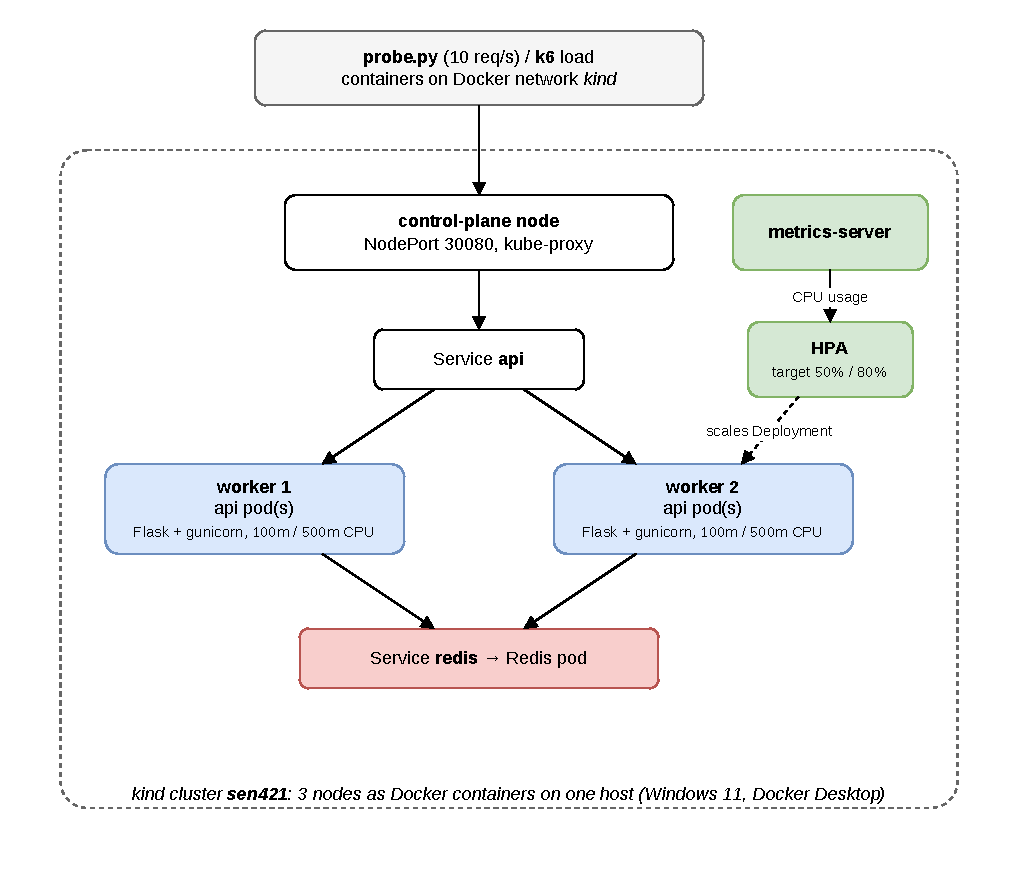
\includegraphics[width=\linewidth]{architecture}}{%
	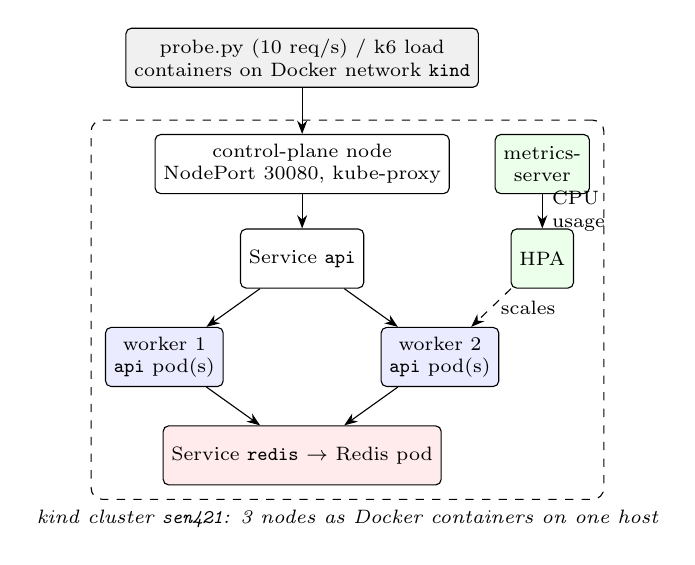
\begin{tikzpicture}[font=\scriptsize, >=Stealth,
		box/.style={draw, rounded corners=2pt, align=center, minimum height=0.75cm, inner sep=3pt, fill=white}]
		\node[box, fill=gray!12] (cl) at (0,0) {probe.py (10 req/s) / k6 load\\containers on Docker network \texttt{kind}};
		\node[box] (np) at (0,-1.35) {control-plane node\\NodePort 30080, kube-proxy};
		\node[box] (svc) at (0,-2.55) {Service \texttt{api}};
		\node[box, fill=blue!8] (w1) at (-1.75,-3.8) {worker 1\\\texttt{api} pod(s)};
		\node[box, fill=blue!8] (w2) at (1.75,-3.8) {worker 2\\\texttt{api} pod(s)};
		\node[box, fill=red!8] (rs) at (0,-5.05) {Service \texttt{redis} $\rightarrow$ Redis pod};
		\node[box, fill=green!8] (ms) at (3.05,-1.35) {metrics-\\server};
		\node[box, fill=green!8] (hpa) at (3.05,-2.55) {HPA};
		\draw[->] (cl) -- (np);
		\draw[->] (np) -- (svc);
		\draw[->] (svc) -- (w1);
		\draw[->] (svc) -- (w2);
		\draw[->] (w1) -- (rs);
		\draw[->] (w2) -- (rs);
		\draw[->] (ms) -- node[right, align=left] {CPU\\usage} (hpa);
		\draw[->, dashed] (hpa) -- node[right] {scales} (w2);
		\node[draw, dashed, rounded corners, fit=(np)(w1)(w2)(rs)(ms)(hpa), inner sep=5pt,
			label={[font=\scriptsize\itshape]below:kind cluster \texttt{sen421}: 3 nodes as Docker containers on one host}] {};
	\end{tikzpicture}}
	\caption{Architecture of the test setup.}
	\label{fig:architecture}
\end{figure}

\subsection{Alternatives Compared}
Table~\ref{tab:alternatives} lists the two alternatives of each experiment. In E1, the baseline is the simplest possible Deployment, one replica without probes, and the hardened variant has three replicas spread over the two workers, readiness and liveness probes, and a 3\,s \texttt{preStop} delay so that a terminating pod is removed from the Service before it stops (Listing~\ref{lst:hardened}). E2 isolates the update strategy: both variants use the hardened pod template and differ only in \texttt{strategy}. E3 compares two HPA targets on the same Deployment (1 to 10 replicas, scale-down window shortened to 60\,s so that scale-in fits into a run).

\begin{lstlisting}[language=bash, float=tb, caption={Excerpt of k8s/api-hardened.yaml}, label={lst:hardened}]
replicas: 3
strategy:
  type: RollingUpdate
  rollingUpdate: { maxSurge: 1, maxUnavailable: 0 }
readinessProbe:
  httpGet: { path: /health, port: 8080 }
  periodSeconds: 1
  failureThreshold: 1
livenessProbe:
  httpGet: { path: /health, port: 8080 }
  initialDelaySeconds: 10
  periodSeconds: 5
lifecycle:
  preStop: { exec: { command: ["sleep", "3"] } }
\end{lstlisting}

\begin{table}[htbp]
	\caption{Alternatives Compared in Each Experiment}
	\label{tab:alternatives}
	\centering
	\footnotesize
	\begin{tabular}{|>{\raggedright\arraybackslash}p{0.13\linewidth}|>{\raggedright\arraybackslash}p{0.35\linewidth}|>{\raggedright\arraybackslash}p{0.35\linewidth}|}
		\hline
		\textbf{Exp.} & \textbf{Alternative A} & \textbf{Alternative B} \\
		\hline
		E1 pod failure & Baseline: 1 replica, no probes & Hardened: 3 replicas, readiness + liveness probes, topology spread \\
		\hline
		E2 update v1$\rightarrow$v2 & Recreate (3 replicas, probes) & RollingUpdate, maxSurge 1, maxUnavailable 0 (3 replicas, probes) \\
		\hline
		E3 load & HPA, 80\,\% CPU target & HPA, 50\,\% CPU target \\
		\hline
	\end{tabular}
\end{table}

kind was chosen because Topic 8 allows a local cluster, it runs a real multi-node Kubernetes (the same API server, scheduler, controllers and kube-proxy as a cloud cluster) and it costs nothing, so the experiments could be repeated as often as needed without billing risk. Because a local cluster has no price, the cost of the same design is estimated for AKS, the managed Kubernetes service of the Azure for Students subscription available to the author; no Azure resources were created.

\subsection{Requirements and Responsibilities}
The availability requirement used for judging the alternatives is that a single pod failure or a planned version update must not cause failed user requests. With kind, the operator is responsible for everything: the nodes, the control plane, Kubernetes upgrades, the container images and the workload configuration. On a managed service such as AKS, the provider operates the control plane and supplies patched node images, and a financially backed uptime SLA for the API server is offered only in the paid Standard tier~\cite{aksTiers}. The customer remains responsible for the workload itself: replicas, probes, update strategy and resource requests, as well as access control (RBAC), network policies, image vulnerabilities, secrets and data~\cite{azshared}. All settings compared in this study are therefore on the customer's side of the shared responsibility model, so a managed service would not remove the downtime measured here.

\section{Methodology}
\label{sec:methodology}

\subsection{Environment}
Table~\ref{tab:environment} lists the environment. Every alternative was run three times; between runs the Deployment was deleted and recreated so that each run started from the same state.

\begin{table}[htbp]
	\caption{Experimental Environment}
	\label{tab:environment}
	\centering
	\footnotesize
	\begin{tabular}{|l|>{\raggedright\arraybackslash}p{0.55\linewidth}|}
		\hline
		\textbf{Property} & \textbf{Value} \\
		\hline
		Platform & Local kind cluster, cost USD 0 \\
		\hline
		Host & Windows 11, 20 logical CPUs, 16 GB RAM, Docker Desktop 29.5.3 \\
		\hline
		Kubernetes & v1.37.0 (kind 0.33.0), 1 control-plane + 2 worker nodes, metrics-server 0.8.0 \\
		\hline
		Application & Flask API on gunicorn (1 worker, 4 threads), Redis 7.4; 3 s warm-up \\
		\hline
		Pod resources & request 100m CPU / 64 MiB, limit 500m / 256 MiB \\
		\hline
		Availability probe & Python client, 1 request per 100 ms, 1 s timeout \\
		\hline
		Load tool (E3) & k6 2.4.0, constant arrival rate 7 req/s on a 50 ms CPU endpoint, 180 s load + 180 s idle \\
		\hline
		Repetitions & 3 per alternative (18 runs in total) \\
		\hline
	\end{tabular}
\end{table}

\subsection{Experiment Procedures}
\textbf{E1} starts the probe, waits until it receives only successful answers, deletes one API pod with \texttt{kubectl delete pod} and records for 45\,s (450 requests). \textbf{E2} starts from three ready v1 pods and changes the image to v2 with \texttt{kubectl set image}; the probe calls \texttt{/version}, so every answer shows which version served it. \textbf{E3} starts from one ready replica, applies the HPA, waits 30\,s and then sends a constant 7 requests per second to \texttt{/cpu} for 180\,s, followed by 180\,s without load. Replica counts and the HPA's utilisation reading are sampled every 2\,s.

\subsection{Measurements}
A request counts as \emph{failed} if it returns a status other than 200 or no answer within 1\,s. \emph{Downtime} is the time from the start of the first failed request to the end of the last failed one, i.e.\ the period in which a user could see errors. In E1, the \emph{Kubernetes-reported recovery} is the time from the delete command until the replacement pod has the condition \texttt{Ready}, polled every 0.2\,s; comparing it with the downtime shows whether Kubernetes' view matches the user's. In E2, the \emph{rollout time} runs from \texttt{set image} until \texttt{kubectl rollout status} returns, and the \emph{mixed-version window} from the first v2 answer to the last v1 answer. In E3, the \emph{first scale-out} is the time from load start until a second replica is ready, \emph{time to max} until the highest replica count is reached, and \emph{scale-in} the time from the end of the load until the Deployment is back at one replica. Latency percentiles (p50, p95) come from k6. \emph{Pod-seconds} is the integral of the number of replicas over the 360\,s run and is used as a proxy for resource cost.

The actual cost is USD 0. The estimated cost uses pay-as-you-go list prices for the Germany West Central region from the Azure Retail Prices API~\cite{azprices}, accessed on 17 November 2026 and stored in the repository, with 730 hours per month.

\subsection{Measurement Path and Validity}
\label{sec:validity}
The first E1 runs used a probe on the Windows host that called \texttt{127.0.0.1:8080}, which Docker Desktop forwards into the control-plane container. These runs showed about 20\,s of failures after a pod deletion. At the same time, \texttt{curl} from inside the node against the pod IP and the NodePort showed that the service had recovered after about 5\,s, so roughly 16\,s of the observed outage was caused by Docker Desktop's port forwarding and not by Kubernetes. All reported results therefore use clients running as containers on the \texttt{kind} network; the affected runs are kept in the repository as evidence but not used. The clocks of the host and the containers were compared before the runs, and their offset was below the 0.25\,s resolution of the check.

A second issue appeared in E3. At 10 requests per second, the demand (about 500\,m CPU) equalled the pod's CPU limit. The single pod became overloaded, its readiness probe timed out, and because the HPA ignores the metrics of pods that are not ready, it never scaled out (Section~\ref{sec:discussion}). These runs are kept separately, and the reported E3 runs use 7 requests per second (about 350\,m, 70\,\% of the limit and 350\,\% of the request).

\subsection{Reproducibility}
All manifests, scripts, raw data and the analysis code are in the repository listed in the Appendix; \texttt{README.md} gives the exact commands. Each experiment script runs three repetitions of both alternatives, and \texttt{analysis/analyze.py} regenerates every table and figure from the raw CSV files.

\section{Results}
\label{sec:results}

\subsection{E1: Pod Failure}
\begin{table}[htbp]
	\caption{E1 Pod Deletion (Mean $\pm$ Std over 3 Runs)}
	\label{tab:e1}
	\centering
	\footnotesize
	\begin{tabular}{|l|c|c|c|}
		\hline
		\textbf{Variant} & \textbf{Failed req.} & \textbf{Downtime (s)} & \textbf{K8s Ready (s)} \\
		\hline
		Baseline & 5.0 $\pm$ 0.0 & 3.21 $\pm$ 0.00 & 0.79 $\pm$ 0.01 \\
		\hline
		Hardened & 0 & 0 & 4.42 $\pm$ 0.04 \\
		\hline
	\end{tabular}
\end{table}

\begin{figure}[htbp]
	\centering
	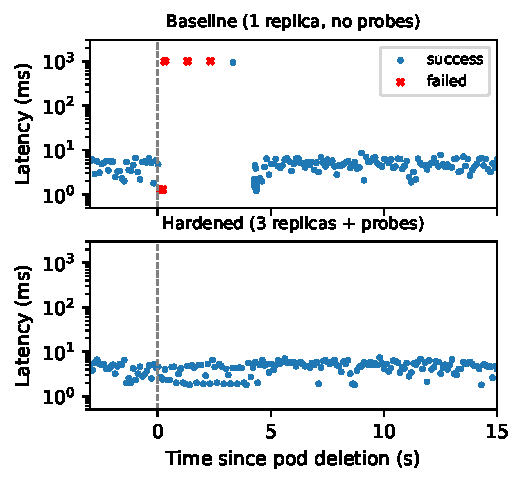
\includegraphics[width=\linewidth]{e1_timeline}
	\caption{Probe requests around the pod deletion at $t=0$ (run 1). Red crosses are failed requests.}
	\label{fig:e1}
\end{figure}
Table~\ref{tab:e1} shows that the baseline lost five of 450 requests in every run, corresponding to 3.21\,s of downtime, with almost no variation between runs. Kubernetes reported the replacement pod as ready after only 0.79\,s, about 2.4\,s before users were served again. Because the baseline has no readiness probe, the pod was marked ready as soon as its container started, while the application was still in its 3\,s warm-up; during this time the Service sent requests to a pod that could not answer them (Fig.~\ref{fig:e1}). The hardened variant had no failed request in any run. Its replacement pod needed 4.42\,s to become ready, longer than in the baseline because the readiness probe waited for the application, but the two remaining replicas served all requests during that time.

\subsection{E2: Version Update}
\begin{table}[htbp]
	\caption{E2 Update v1$\rightarrow$v2 (Mean $\pm$ Std over 3 Runs)}
	\label{tab:e2}
	\centering
	\footnotesize
	\setlength{\tabcolsep}{3pt}
	\begin{tabular}{|l|c|c|c|c|}
		\hline
		\textbf{Strategy} & \textbf{Rollout (s)} & \textbf{Failed} & \textbf{Downtime (s)} & \textbf{Mixed (s)} \\
		\hline
		Recreate & 7.85 $\pm$ 0.21 & 14.3 $\pm$ 2.5 & 5.37 $\pm$ 0.16 & 0 \\
		\hline
		RollingUpdate & 12.41 $\pm$ 0.15 & 0 & 0 & 8.33 $\pm$ 0.31 \\
		\hline
	\end{tabular}
\end{table}

\begin{figure}[htbp]
	\centering
	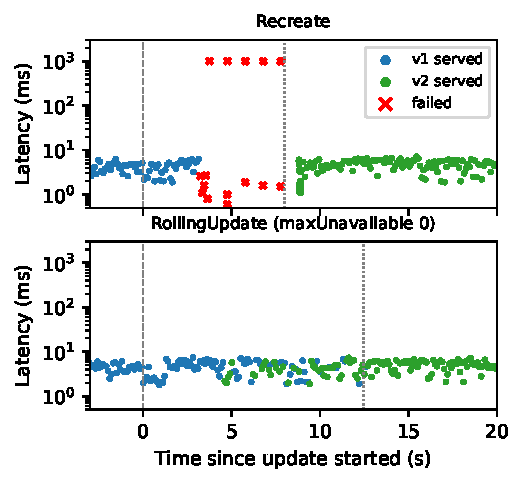
\includegraphics[width=\linewidth]{e2_timeline}
	\caption{Version served and latency during the update (run 1). Dashed line: update starts; dotted line: rollout complete.}
	\label{fig:e2}
\end{figure}
With \texttt{Recreate}, every update caused 5.37\,s of downtime and on average 14.3 failed requests (Table~\ref{tab:e2}): all three v1 pods were terminated before any v2 pod existed, and the v2 pods then needed their 3\,s warm-up. \texttt{RollingUpdate} caused no failed requests in any run. It was, however, 4.6\,s (58\,\%) slower, because it replaced the pods one at a time and waited for each new pod to become ready. For 8.33\,s, both versions answered requests at the same time (Fig.~\ref{fig:e2}). Apart from the outage, latency was not affected: the p95 latency of successful requests was about 6\,ms before and during the update for both strategies.

\subsection{E3: Horizontal Pod Autoscaling}
\begin{table}[htbp]
	\caption{E3 HPA at 7 req/s on /cpu (Mean $\pm$ Std over 3 Runs)}
	\label{tab:e3}
	\centering
	\footnotesize
	\begin{tabular}{|l|c|c|}
		\hline
		\textbf{Metric} & \textbf{HPA 80\%} & \textbf{HPA 50\%} \\
		\hline
		First scale-out (s) & 35.2 $\pm$ 15.7 & 34.9 $\pm$ 0.2 \\
		\hline
		Max replicas & 5.3 $\pm$ 0.6 & 9.3 $\pm$ 1.2 \\
		\hline
		Time to max (s) & 45.4 $\pm$ 18.0 & 70.6 $\pm$ 23.2 \\
		\hline
		Scale-in after load (s) & 85.7 $\pm$ 8.6 & 91.0 $\pm$ 0.5 \\
		\hline
		p50 latency (ms) & 61.1 $\pm$ 6.2 & 62.3 $\pm$ 6.6 \\
		\hline
		p95 latency (ms) & 118.2 $\pm$ 19.5 & 111.9 $\pm$ 6.1 \\
		\hline
		Failed requests & 0 & 0 \\
		\hline
		Pod-seconds per run & 1323 $\pm$ 99 & 2090 $\pm$ 146 \\
		\hline
	\end{tabular}
\end{table}
\begin{figure}[htbp]
	\centering
	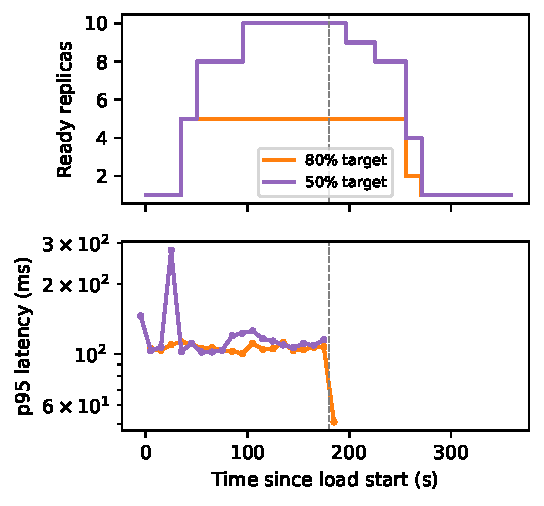
\includegraphics[width=\linewidth]{e3_hpa}
	\caption{Ready replicas and p95 latency per 10 s window (run 1). Dashed line: load stops.}
	\label{fig:e3}
\end{figure}
Under the same load, both targets added the first replica after about 35\,s (Table~\ref{tab:e3}). This delay consists of the 15\,s metrics resolution, the 15\,s HPA interval and the warm-up of the new pod. The HPA measured about 390\,\% utilisation of the CPU request and scaled the 80\,\% variant to 5--6 replicas and the 50\,\% variant to 8--10 replicas, as expected from the HPA formula. The 80\,\% target reached its maximum sooner because it needed fewer steps. After the load stopped, both returned to one replica within about 90\,s, i.e.\ the 60\,s stabilisation window plus the metrics delay (Fig.~\ref{fig:e3}). No request failed, and median and p95 latency were almost the same for both targets. The large spread of the 80\,\% target comes from run 3, where the first scale-out took 51\,s and the p95 latency in the first minute reached 531\,ms instead of about 110\,ms. The 50\,\% target consumed 58\,\% more pod-seconds.

\subsection{Cost Results}
The experiments ran on a local cluster, so the \textbf{actual cost was USD 0}, and no cloud resources were created that would need deleting. Table~\ref{tab:cost} estimates the monthly cost of running the two E1 alternatives on AKS. The baseline uses the Free control-plane tier and one B2s node; the hardened variant uses the Standard tier, which includes the uptime SLA~\cite{aksTiers}, and three B2s nodes so that the three replicas can be placed on separate machines. Data transfer and load balancer rules were not included.

\begin{table}[htbp]
	\caption{Estimated Monthly AKS Cost, Germany West Central (USD)}
	\label{tab:cost}
	\centering
	\footnotesize
	\begin{tabular}{|l|c|c|}
		\hline
		\textbf{Cost item} & \textbf{Baseline} & \textbf{Hardened} \\
		\hline
		Control plane (Free / Standard tier) & 0.00 & 73.00 \\
		\hline
		Compute (B2s, 1 / 3 nodes) & 35.04 & 105.12 \\
		\hline
		OS disks (E10, 1 / 3) & 9.60 & 28.80 \\
		\hline
		Public IP & 3.65 & 3.65 \\
		\hline
		\textbf{Total} & \textbf{48.29} & \textbf{210.57} \\
		\hline
	\end{tabular}
\end{table}
The hardened setup costs 4.4 times as much, USD 162.28 more per month. For E3, the CPU requested by the pods during one load burst was priced at the B2s price per vCPU (USD 0.024 per vCPU-hour). One burst cost USD 0.00139 with the 50\,\% target and USD 0.00088 with the 80\,\% target; with one such burst per hour this is USD 1.02 compared with USD 0.64 per month. Neither E2 alternative needs extra nodes; RollingUpdate only needs room for one additional pod during the update.

\section{Discussion}
\label{sec:discussion}
In both E1 and E2, the hardened configuration met our reliability requirement with zero failed requests, whereas the baseline configuration fell short. However, this reliability comes at a financial cost, as the hardened setup is roughly 162 USD more expensive per month on AKS (USD 211 vs.\ USD 48). Whether this extra expense is justified depends entirely on the business impact of downtime; a three-second disruption might be acceptable for an internal tool, while it would be unacceptable for a payment processing system. Additionally, our cost comparison might exaggerate the difference when applied to larger production environments. In practice, running three replicas does not necessarily require three separate virtual machines, and the fixed fee for the AKS Standard tier is distributed across all applications sharing the cluster.

One of the most surprising results was how misleading the ``Ready'' status can be when a readiness probe is missing. Without a probe, Kubernetes marked the newly created pod as ready in just 0.8 seconds, yet users continued to experience failed requests for 3.2 seconds. From Kubernetes' perspective, self-healing worked immediately, even though the service remained unavailable from the user's perspective. Simply put, Kubernetes cannot know an application is truly ready to serve traffic unless the application explicitly reports it. On the other hand, there is a trade-off: because our \texttt{/health} endpoint also checks the Redis connection, a Redis failure would cause all pods to be removed from traffic. While this behavior makes sense for our application since it cannot function without Redis, it might not be the right approach for every system.

Using the RollingUpdate strategy eliminated downtime completely, though it came with hidden operational requirements. The update process took 58\,\% longer to complete (12.41 seconds compared to 7.85 seconds), and both v1 and v2 versions served traffic simultaneously for over eight seconds. During this transition window, a client might receive a response from v2 on one request and from v1 on the next. Therefore, both versions must remain strictly compatible in terms of database schemas and API formats. In contrast, the Recreate strategy is much simpler and remains a practical choice when two versions cannot coexist and a brief, planned outage is acceptable.

Our autoscaling experiments highlighted both the impact of CPU target thresholds and a critical overload trap. Since CPU utilization is calculated relative to the pod's CPU request, the exact same workload scaled up to 5 pods at an 80\,\% target versus 9 pods at a 50\,\% target. Despite this difference, p95 latency remained nearly identical (118\,ms vs.\ 112\,ms), meaning the 80\,\% target was sufficient for this load while consuming 37\,\% less pod-time. The main advantage of the lower 50\,\% target is scaling out earlier, which was evident when the 80\,\% target's third run saw p95 latency spike to 531\,ms during the first minute. More importantly, the 10 requests-per-second overload test exposed a major failure mode: the single pod became saturated, its readiness probe failed, and the Horizontal Pod Autoscaler (HPA) ignored the unready pod instead of scaling up, resulting in 405 to 673 failed requests. Because the autoscaler failed at the exact moment it was needed most, our key takeaway is to set \texttt{minReplicas} to at least 2 and configure CPU requests to accurately match real workload needs.

Migrating to a managed service like AKS shifts the management of the control plane and node images to Microsoft under the shared responsibility model~\cite{azshared}. However, none of the reliability issues we observed fall under the cloud provider's responsibility; configuring replicas, health probes, update strategies, and HPA thresholds remains entirely up to the user. While our setup avoided hardcoded secrets and used the official \texttt{python:3.12-slim} base image, it lacked RBAC restrictions, NetworkPolicies, container image scanning, and Redis authentication. These omissions are acceptable for a local experiment, but they must be addressed before moving to production. Similarly, regarding data privacy regulations like KVKK, our tests relied solely on synthetic data, whereas handling real personal data would require careful consideration of data center regions and cross-border data transfer rules.

Finally, several limitations should be kept in mind when interpreting these results. All cluster nodes ran on a single physical machine, meaning our fault injection simulated pod deletions rather than actual hardware or node failures, and the load generation tools shared the same CPU resources as the cluster. Furthermore, both the application and traffic patterns were synthetic, with each test repeated three times over relatively short durations. Our cost estimates are also based on standard list prices without accounting for discounts, taxes, or data transfer fees. Lastly, the measurement path issue we encountered demonstrated how the method of observation alone can skew results by several multiples, such as measuring 20 seconds instead of 5 seconds.

\section{Conclusion and Future Work}
\label{sec:conclusion}
Overall, moving from the baseline to the hardened configuration reduced user-facing downtime from 3.2 seconds to 0 seconds during pod failures and from 5.4 seconds to 0 seconds during updates, though updates took 58\,\% longer to finish. In autoscaling tests, both CPU targets triggered the first scale-up at around 35 seconds, with the 50\,\% target consuming 58\,\% more pod-time, while the single-pod overload scenario failed to scale at all. Based on these findings, we recommend deploying at least three replicas, configuring proper readiness probes, using RollingUpdate with backward-compatible versions, and setting HPA targets around 70--80\,\% with \texttt{minReplicas} set to at least 2 --- a setup that costs roughly four times more on AKS. The primary lesson from this study is that while Kubernetes provides powerful reliability mechanisms out of the box, achieving actual resilience requires careful tuning and measuring impact directly from the user's perspective. Future work should expand on these tests by deploying across multiple availability zones on AKS, simulating full node shutdowns, and evaluating PodDisruptionBudget, startup probes, and the cluster autoscaler under longer, more realistic workloads.

\section*{AI Tool Use and Originality Declaration}
\label{sec:ai_declaration}
AI-assisted tools (Claude, Anthropic) were used extensively in this project: for planning the experiments and wording the research question, suggesting documentation sources, writing and debugging the Kubernetes manifests, experiment scripts and analysis code, diagnosing the measurement-path and HPA overload issues, fetching list prices from the official Azure Retail Prices API, and drafting the text of most sections of this report. The Discussion and Conclusion were written by the student from an AI-provided outline of the points to cover; the AI then only checked grammar and numbers. The student chose the topic, ran all experiments on their own machine, checked every reported number against the raw data in the repository, and reviewed and approved the final text. All numbers come from real runs. The student accepts full responsibility for the accuracy, originality, reproducibility and integrity of the submitted work. Table~\ref{tab:ai_use} summarises the level of AI support per project stage.

\begin{table}[htbp]
	\caption{AI Use Disclosure Summary}
	\label{tab:ai_use}
	\centering
	\footnotesize
	\begin{tabular}{|>{\raggedright\arraybackslash}p{0.40\linewidth}|c|>{\raggedright\arraybackslash}p{0.38\linewidth}|}
		\hline
		\textbf{Project Stage} & \textbf{Level} & \textbf{Brief Description} \\
		\hline
		Topic and question & 3 & Student's topic; wording refined with AI \\
		\hline
		Literature and documentation search & 3 & AI suggested sources \\
		\hline
		Design, deployment, and configuration & 4 & AI wrote manifests, scripts \\
		\hline
		Measurement, cost analysis, and modeling & 4 & AI wrote analysis code; student ran it \\
		\hline
		Writing, editing, and LaTeX formatting & 5 & Sections I--V drafted by AI, reviewed by student \\
		\hline
		Interpretation, discussion, and conclusion & 3 & Written by student from an AI outline; AI checked grammar \\
		\hline
	\end{tabular}
\end{table}

\begin{thebibliography}{00}
\bibitem{nist} P.~Mell and T.~Grance, ``The NIST definition of cloud computing,'' National Institute of Standards and Technology, Gaithersburg, MD, USA, NIST Special Publication 800-145, 2011.
\bibitem{west} J.~West, \textit{CompTIA Cloud+ Guide to Cloud Computing}, 2nd~ed. Boston, MA, USA: Cengage, 2024.
\bibitem{borg} B.~Burns, B.~Grant, D.~Oppenheimer, E.~Brewer, and J.~Wilkes, ``Borg, Omega, and Kubernetes,'' \textit{Communications of the ACM}, vol.~59, no.~5, pp.~50--57, May 2016.
\bibitem{k8sdeploy} The Kubernetes Authors, ``Deployments,'' Kubernetes Documentation. [Online]. Available: \url{https://kubernetes.io/docs/concepts/workloads/controllers/deployment/}. [Accessed: 17 Nov. 2026].
\bibitem{k8sprobes} The Kubernetes Authors, ``Configure liveness, readiness and startup probes,'' Kubernetes Documentation. [Online]. Available: \url{https://kubernetes.io/docs/tasks/configure-pod-container/configure-liveness-readiness-startup-probes/}. [Accessed: 17 Nov. 2026].
\bibitem{k8shpa} The Kubernetes Authors, ``Horizontal pod autoscaling,'' Kubernetes Documentation. [Online]. Available: \url{https://kubernetes.io/docs/tasks/run-application/horizontal-pod-autoscale/}. [Accessed: 17 Nov. 2026].
\bibitem{kind} The Kubernetes Authors, ``kind --- Kubernetes in Docker.'' [Online]. Available: \url{https://kind.sigs.k8s.io/}. [Accessed: 17 Nov. 2026].
\bibitem{aksTiers} Microsoft, ``Free, Standard, and Premium pricing tiers for Azure Kubernetes Service (AKS) cluster management,'' Microsoft Learn. [Online]. Available: \url{https://learn.microsoft.com/en-us/azure/aks/free-standard-pricing-tiers}. [Accessed: 17 Nov. 2026].
\bibitem{azshared} Microsoft, ``Shared responsibility in the cloud,'' Microsoft Learn. [Online]. Available: \url{https://learn.microsoft.com/en-us/azure/security/fundamentals/shared-responsibility}. [Accessed: 17 Nov. 2026].
\bibitem{azprices} Microsoft, ``Azure Retail Prices REST API overview,'' Microsoft Learn. [Online]. Available: \url{https://learn.microsoft.com/en-us/rest/api/cost-management/retail-prices/azure-retail-prices}. [Accessed: 17 Nov. 2026].
\end{thebibliography}

\appendix
\section{Code Repository}
\label{app:code}
Manifests, scripts, raw results and analysis code: \url{https://github.com/demcan15/sen421-k8s-orchestration}.


\end{document}
